\documentclass[a4paper, 12pt, titlepage]{article}

\usepackage[utf8]{inputenc}
\usepackage{geometry}
\usepackage{graphicx}
\usepackage{float}
\usepackage{etoolbox,refcount}
\usepackage{multicol}
\usepackage{fancyhdr}
\usepackage{listings}
\usepackage{amsmath}
\usepackage{tabularx}
\usepackage{svg}
\usepackage{fancyhdr}

\pdfsuppresswarningpagegroup=1
\newgeometry{left=3cm, right=3cm, bottom=3cm, top=3cm}

\lstset{
    language=Ada,
    basicstyle=\ttfamily,
    keepspaces=true,
    frame=single,
    tabsize=4,
    showspaces=false,
    showstringspaces=false,
    extendedchars=true,
    inputencoding=utf8,
}

\pagestyle{fancy}
\title{The implementation of ``Walking One'' algorithm at SIEMENS 1200 \\
Hardware and Software of Control Systems}
\author{Adrian Jałoszewski \\ \\
    Faculty: EAIiIB, \\
    Speciality: ISZ, \\
    Group: 1, \\
    Instructor: mgr inż. Klaudia Dziedzic}
\date{Submision date: 08.12.2017}

\begin{document}
    \maketitle
    \tableofcontents 
    \newpage
    \section{Introduction}
        \subsection{Uses of the algorithm}
            The ``walking one'' algorithm is one of the most well known
            algorithms used for testing the independence of operations
            performed by changing the state of consecutive bits.
            \\ \\
            Its primal intention is checking of coupling between two 
            consecutive bits which ideally should be independent. If by
            changing the output by one two of them have the undesired 
            state this means that the input device is not functioning 
            properly.
        \subsection{Hardware description}
            As pointed out in the requirements the picked PLC was: \\ \\
            SIMANTIC S7-1200 1212c DC/DC/DC -- 6ES7 212-1AE40-0xB0 -- Firmware V4.1 
            \\ \\
            Because of the low ammount of digital outputs the following IO module was
            added: \\ \\
            DI 16x24VDC/DQ 16xRelay -- 6ES7 223-1PL30-0XB0 -- Firmware V1.0 \\ \\
            Despite offering more it was used just as a digital output device.
            \begin{figure}[H]
                \centering
                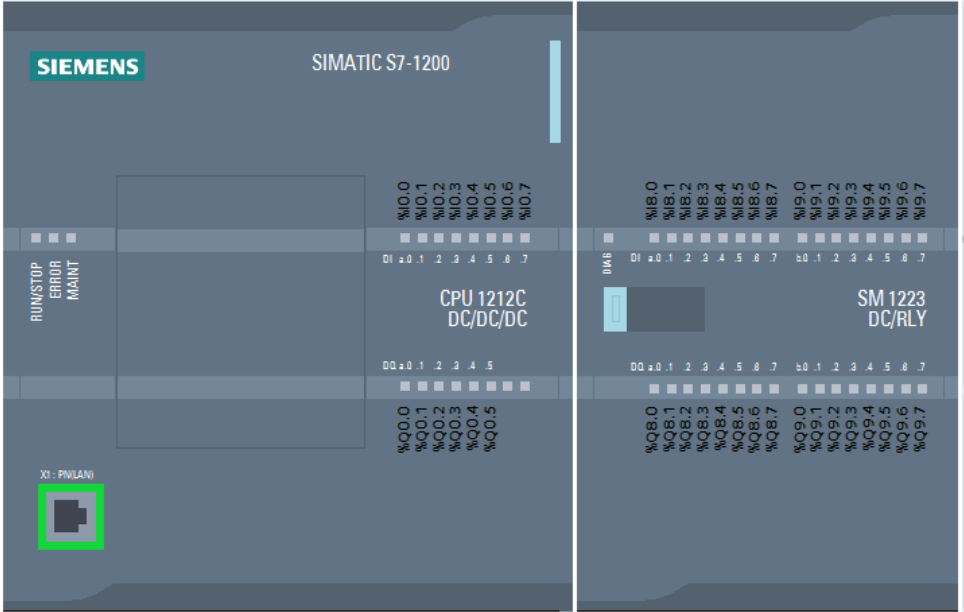
\includegraphics[width=0.9\linewidth]{plc.png}
                \caption{Hardware setup}
            \end{figure}
        \subsection{Specification}
            The requirements tated for the implementation of the algorithm to be
            performed using TIA Portal v13 or v14 with PLCSim. The implementation 
            had to be written using the SCL language with cyclic interrupt Organization
            Blocks, indirect addressing and Function Blocks.
    \section{Algorithm description}
        \begin{figure}[H]
            \centering
            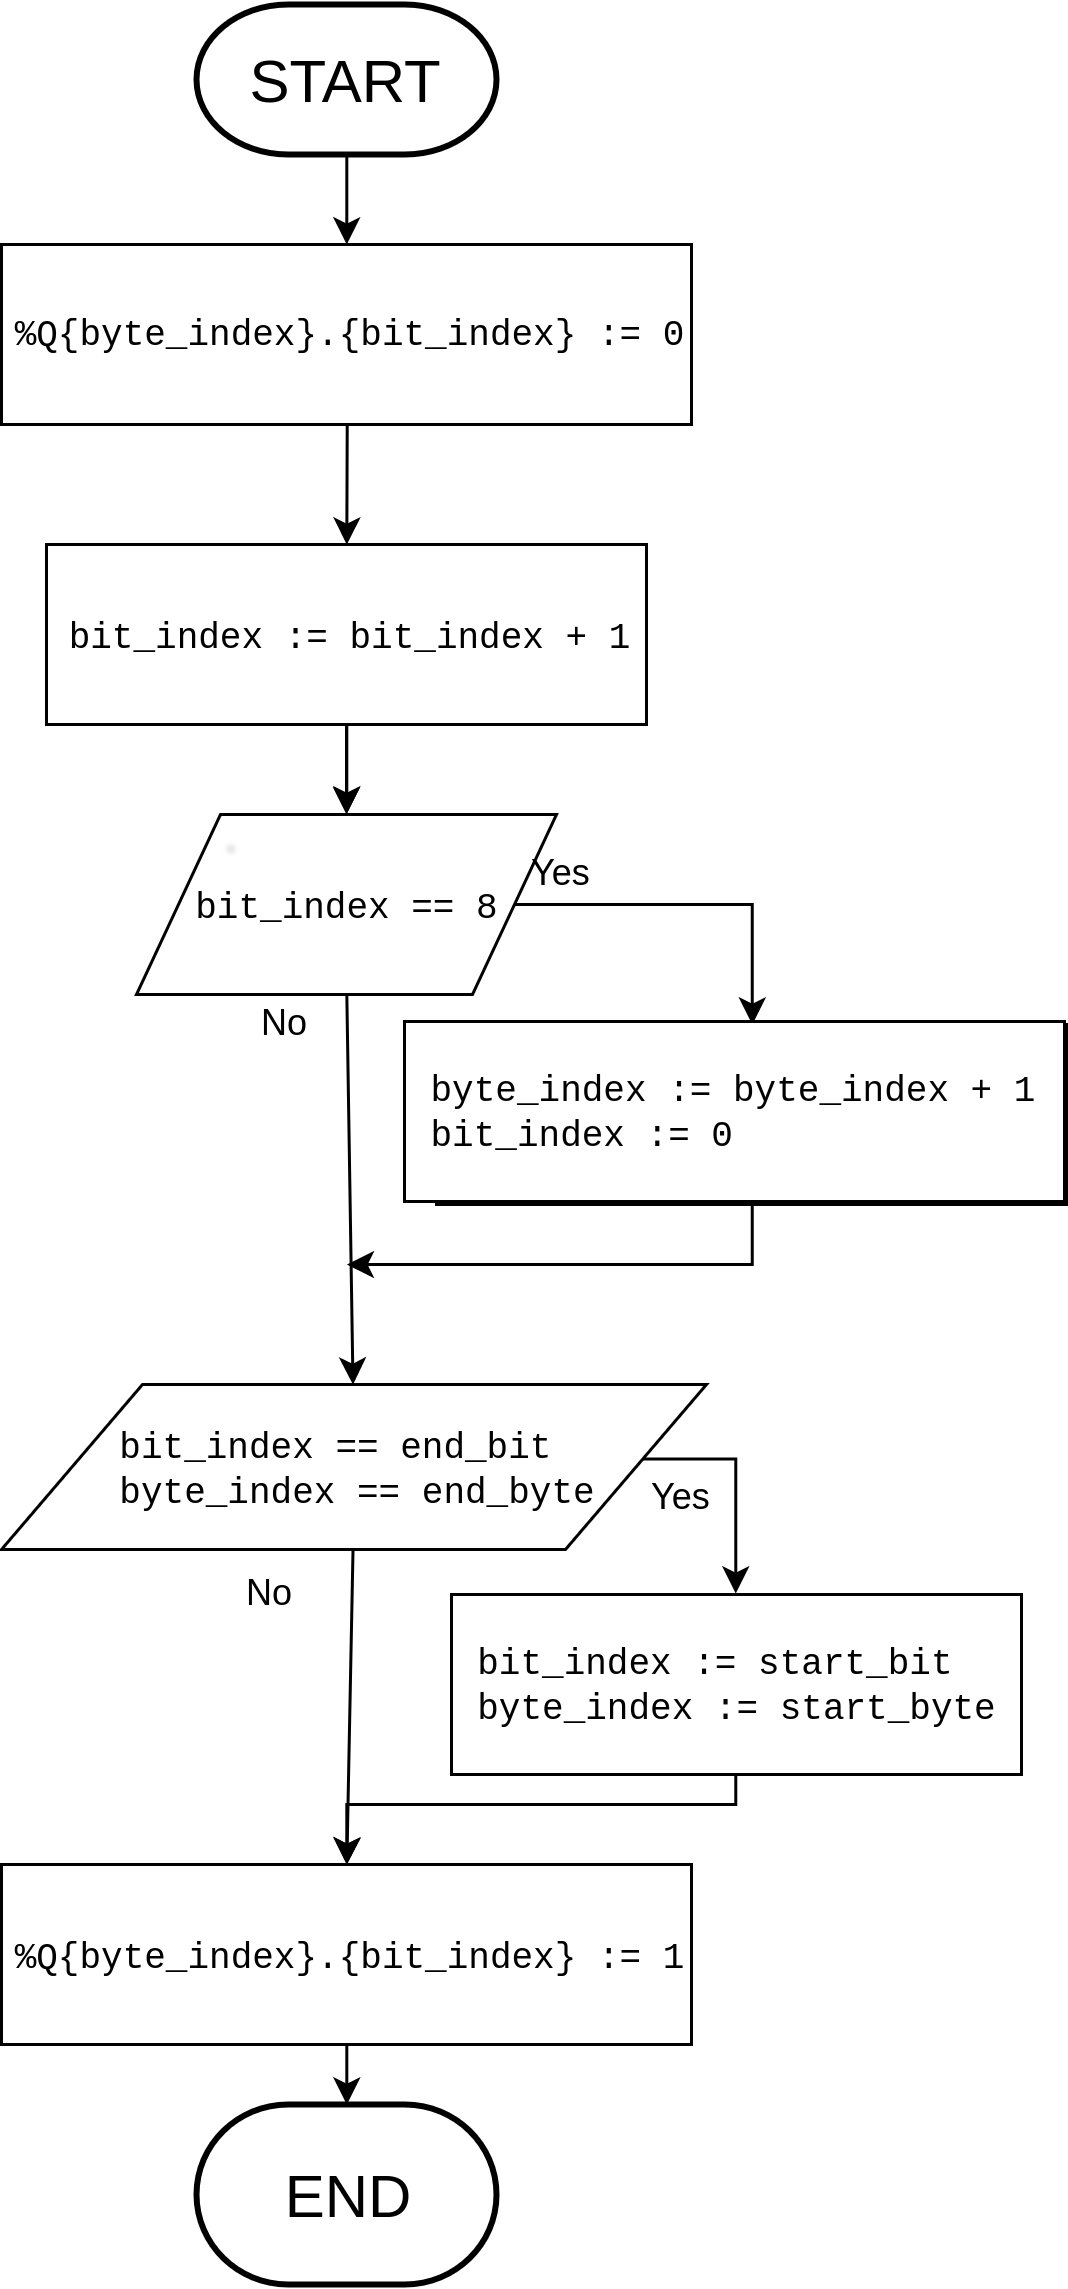
\includegraphics[width=0.5\linewidth]{algo.png}
            \caption{Algorithm flow chart}
        \end{figure}
    \section{Implementation details}
        \subsection{Variables and valueds}
            Because of indirect addressing and the technologies applied all
            the variables and values had to be represented by two numbers --
            the \textbf{\texttt{bitOffset}} and \textbf{\texttt{byteOffset}}.
            Both of them can be put in the output address representation like \linebreak 
            \textbf{\texttt{\%Q\{byteOffset\}.\{bitOffset\}}}. An additional 
            limitation to the \textbf{\texttt{bitOffset}} is that it can only
            be in range of 0 to 7. All the datatypes were picked to match the 
            ones which were required by the \texttt{\textbf{POKE\_BOOL}} function.

            \subsubsection{Global constants}
                There were four global constants -- all of them were used as
                program constraints. They can be grouped into two parts:
                \begin{itemize}
                    \item The output with the least number:
                        \begin{itemize}
                            \item \textbf{\texttt{start\_byte}} -- \textbf{\texttt{dint}}
                            \item \textbf{\texttt{start\_bit}} -- \textbf{\texttt{int}}
                        \end{itemize}
                    \item The output with the number after the range:
                        \begin{itemize}
                            \item \textbf{\texttt{end\_byte}} -- \textbf{\texttt{dint}} 
                            \item \textbf{\texttt{end\_bit}} -- \textbf{\texttt{int}}
                        \end{itemize}
                \end{itemize}
            \subsubsection{Local variables of function block}
                The function block which was used for this algorithm consists of two
                variables. Both initialized at the beginning to the least alowable
                values. They retain their state between function block calls.
                \begin{itemize}
                    \item[--] \textbf{\texttt{byte\_index}} -- \textbf{\texttt{dint}} 
                    \item[--] \textbf{\texttt{bit\_index}} -- \textbf{\texttt{int}} 
                \end{itemize}
                These are the variables which are updated every interrupt.
        \subsection{Source code}
            Because of the use of \texttt{\textbf{POKE\_BOOL}} the code became platform
            dependent and is not to be reused on other SIEMENS PLCs. The code consists of
            three separate parts:
            \subsubsection{Setting the previous one to zero}
                The following call is responsible for setting the output at 
                \textbf{\texttt{\%Q\{byteOffset\}.\{bitOffset\}}} to zero. 
                \texttt{\textbf{16\#82}} tells the function to look at the output memory
                area to change. The function changes only the bit it is pointed two with the
                two parameters.
\begin{lstlisting} 
POKE_BOOL(area:=16#82,
          bitOffset:=#bit_index,
          byteOffset:=#byte_index,
          dbNumber:= 0,
          value:=FALSE);
\end{lstlisting}
            \subsubsection{Updating the indices}
\begin{lstlisting}
#bit_index := #bit_index + 1;

IF #bit_index = 8 THEN
    #byte_index := #byte_index + 1;
    #bit_index := 0;
END_IF;

IF #byte_index = "end_byte" AND #bit_index = "end_bit" THEN
    #byte_index := "start_byte";
    #bit_index := "start_bit";
END_IF;
\end{lstlisting}
            \subsubsection{Setting the next one}
\begin{lstlisting}
POKE_BOOL(area := 16#82,
          bitOffset := #bit_index,
          byteOffset := #byte_index,
          dbNumber := 0,
          value := TRUE);
\end{lstlisting}
    \section{Simulation}
        The simulated examples contain the full range of corner cases
        which had to be taken into consideration. Considered were
        cases where the limits were set either to values which are the 
        least and highest possible or the cases just before them (one
        above minimum and one below maximum).
        \begin{table}[H]
            \centering
            \caption{Test sets}
            \begin{tabular}{|r|r|r|r|l|} \hline
                \textbf{\texttt{start\_byte}} & \textbf{\texttt{start\_bit}} & 
                \textbf{\texttt{end\_byte}} & \textbf{\texttt{end\_bit}} & 
                Experiment result \\ \hline
                8 & 0 & 10 & 0 & Passed \\ \hline
                8 & 1 & 10 & 0 & Passed \\ \hline
                8 & 0 & 9 & 7 & Passed \\ \hline
                8 & 1 & 9 & 7 & Passed \\ \hline
            \end{tabular}
        \end{table} \noindent
        The only issuse encountered here were that the first iteration
        started at the second cell instead of the first one, but the rest
        continued to work properly. The workaround to that is taking the 
        last indices of the range of intrest as the starting ones -- the 
        last output would be set to zero and the first output set to one
        would be the first one. Working around this behaviour would require
        additional setup logic which should calculate the last valid index
        with all corner cases.
    \section{Summary}
        \subsection{Results obtained}
            The results obtained is a fully functioning walking one implementation
            with a change period of one second. The first iteration warries just 
            a bit from the expected value (it does not pick up the first ouput in
            the first iteratinon), but despite that it works well and does not have
            the same issue in the iterations afterwards.
        \subsection{Difficulties encountered}
            The biggest issue here was with the 21-day trial license. SIEMENS did 
            not handle the usecase when somebody decided to use another trial
            version of their software on the same computer -- after installing TIA
            Portal v14 there were issues with using TIA Portal v13 because it
            recognized the previous license instead of using its own. The solution
            to this problem was installing the software on another computer
            (another would be to completely reinstall the operating system).
            \\ \\
            Another issue was a bug which did not allow running PLCSim because of
            missing DLL -- this required just installing another patch.
        \subsection{Lessons for the future}
            One of the most meaningful lessons was a selfcheck on remembering the 
            process of programming a PLC device, but this time in another language
            and using Organizat Blocks instead of LAD and Function Blocks. 
            \\ \\
            Another lesson was simulating PLC behaviour and the pitfalls of it
            when the configurations of both programmes do not match up.
            \\ \\
            It also showed a effective way of eliminating boilerplate code by using
            excel like sheets for variable declaration (which take less place than
            actual SCL code).
\end{document}
